\begin{atiTask}[
  title = Verifikation des GAUSSschen Satzes
]

Gegeben sei das Vektorfeld
\[
\vec{A}=\frac{6ka^2y}{\sqrt{x^2+y^2+a^2}}\vec{i} +\frac{3ka^2z}{\sqrt{y^2+z^2+4a^2}}\vec{j}+\frac{2ka^2x}{\sqrt{x^2+z^2+9a^2}}\vec{k}
\]
und die Oberfläche eines Quaders, der durch die Eckpunkte der Grundfläche $(0,0,0)$ $(2a,0,0)$, $(2a,3a,0)$, $(0,3a,0)$ und die Höhe $a$ beschrieben wird.
\begin{atiSubtasks}
\item Skizzieren Sie den Quader und die Flächennormalenvektoren.
\item Berechnen Sie den Fluss des Vektorfeldes durch die Oberfläche des Quaders durch Ausführen eines Oberflächenintegrals im Sinne des \textsc{Gauss}schen Satzes.
\item Berechnen Sie den Fluss noch einmal indem Sie über das Volumen des Quaders im Sinne des \textsc{Gauss}schen Satzes integrieren.
\end{atiSubtasks}

\end{atiTask}

\begin{atiSolution}
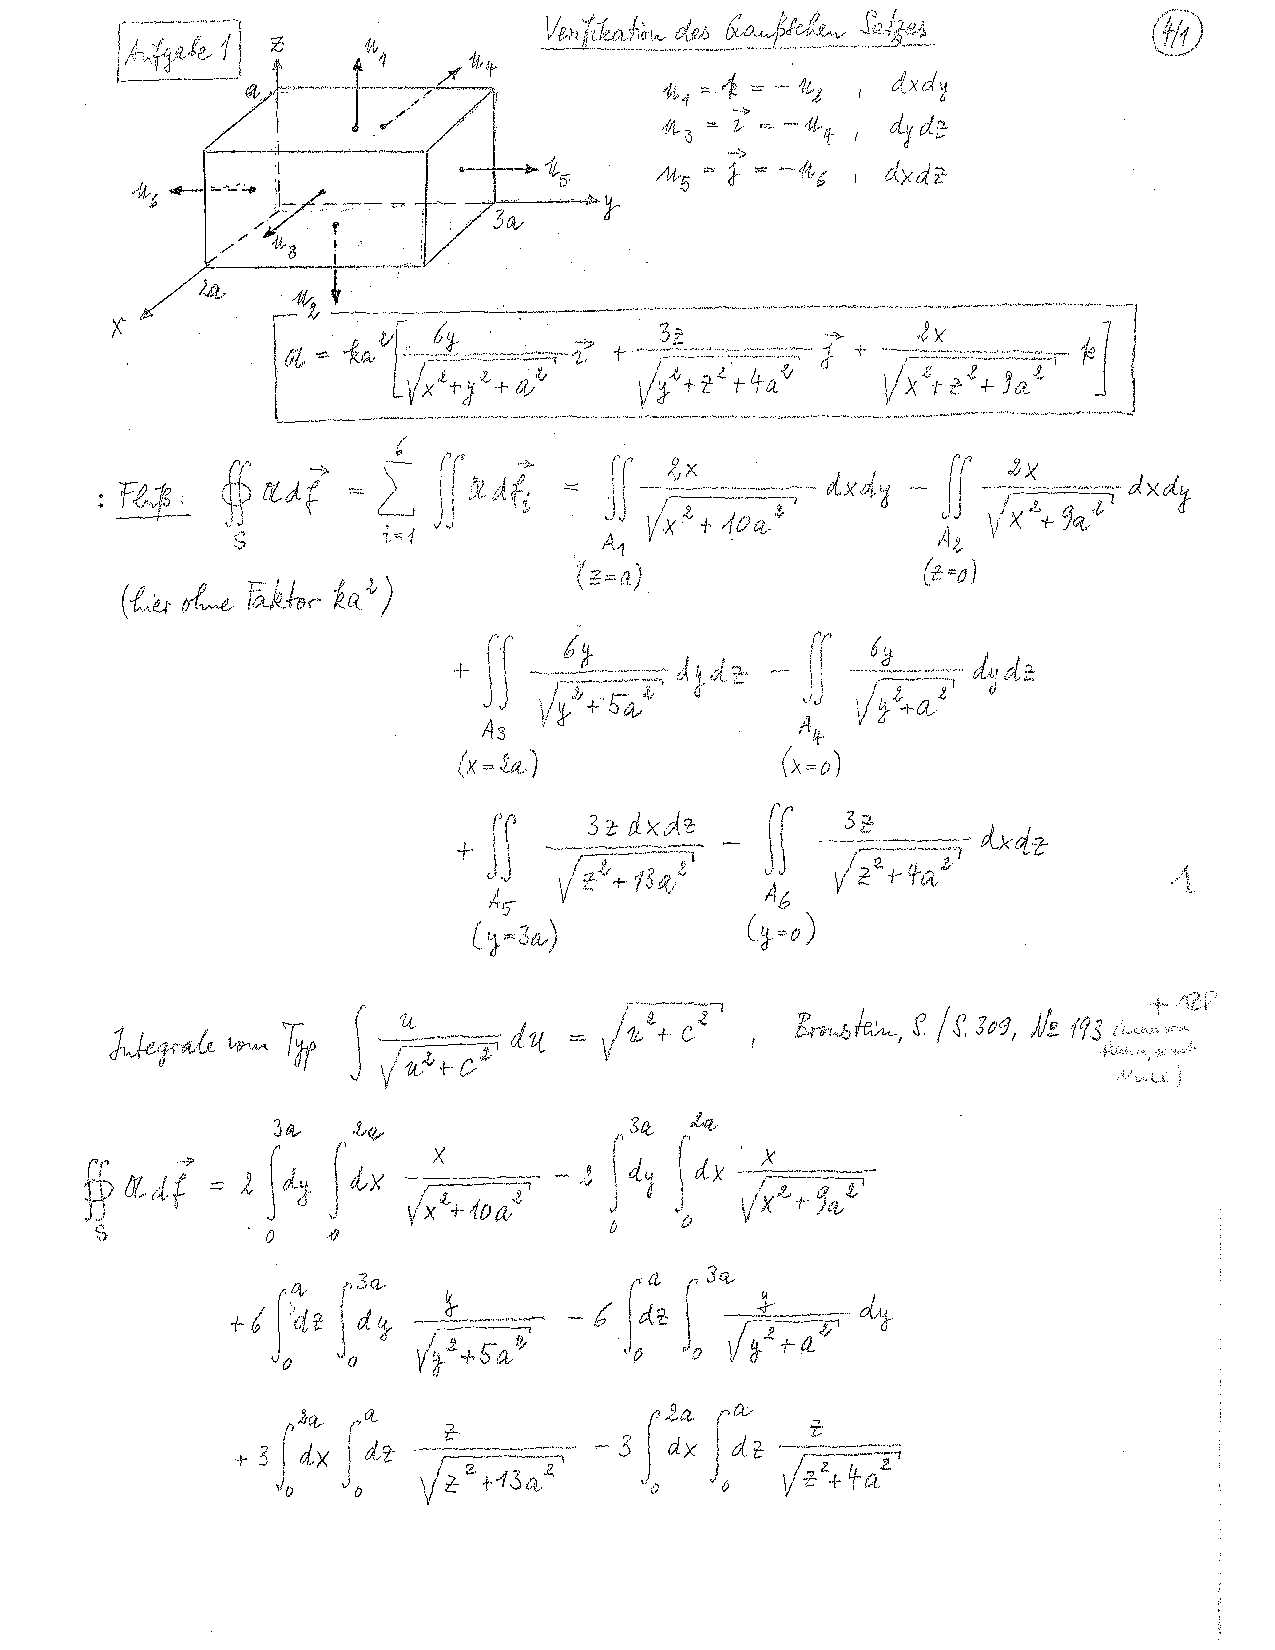
\includepdf[pages=-]{solution-gauss_i.pdf}
\end{atiSolution}
